\documentclass[a4paper,12pt]{article}
\usepackage{standalone}
\usepackage[a4paper, top=0.8in, bottom=0.7in, left=0.8in, right=0.8in]{geometry}
\usepackage{amsmath}
\usepackage{hyperref}
\usepackage{amsfonts}
\usepackage{latexsym}
\usepackage{graphicx}
\usepackage{fancyhdr}
\usepackage{enumitem}
\usepackage{setspace}
\usepackage{tcolorbox}
\usepackage{tikz}
\usepackage{multicol}
\usepackage[defaultfam,tabular,lining]{montserrat} % Font settings for Montserrat

\usepackage{xcolor}  % To use colors
\hypersetup{
    colorlinks=true,   % Activate colored links
    linkcolor=blue,    % Link color for internal links
    urlcolor=blue,     % Link color for URLs
    filecolor=blue,    % Link color for file links
    menucolor=blue,    % Link color for menus
}



\sloppy

\title{}
\date{}
\hyphenpenalty=10000
\exhyphenpenalty=10000

\setlength{\parindent}{0pt}
\pagestyle{fancy}

\setlength{\headheight}{27.11148pt}
\addtolength{\topmargin}{-15.11148pt}

\fancyhf{}
\fancyhead[L]{\textbf{Curriculum D SWB}}
\fancyhead[R]{
\includegraphics[width=0.8cm]{Round Logo.png}} % Placeholder for logo
\fancyfoot[C]{\footnotesize © Study Smart Tutors}
\fancyfoot[R]{\thepage}  % Page number in bottom right corner
\fancyfoot[L]{\hyperlink{toc}{Back to Contents}} % Clickable link in bottom left to TOC




\sloppy

% Define a new command for the level letter
\newcommand{\levelLetter}{D}  % Change this letter to update throughout the document

%%%%%%%%%%%%%%%%%%%%%%%%%%%%%%%%%%%%%

\begin{document}

% Title Page
\documentclass[12pt]{article}
\usepackage[a4paper, top=0.8in, bottom=0.7in, left=0.8in, right=0.8in]{geometry}
\usepackage{amsmath}
\usepackage{amsfonts}
\usepackage{latexsym}
\usepackage{graphicx}
\usepackage{tikz}
\usepackage{fancyhdr}
\usepackage{tcolorbox}
\usepackage{multicol}
\usepackage{tgadventor}
\renewcommand{\familydefault}{\sfdefault}
\usepackage{enumitem}
\usepackage{setspace}
\setlength{\parindent}{0pt}
\pagestyle{fancy}
\usepackage{needspace}


% Define a new command for the level letter
\newcommand{\levelLetter}{D}  % Change this letter to update throughout the document

%%%%%%%%%%%%%%%%%%%%%%%%%%%%%%%%%%%%%

\setlength{\headheight}{27.11148pt}
\addtolength{\topmargin}{-15.11148pt}

\fancyhf{}
%\fancyhead[L]{\textbf{5.NBT.A.1: Understand the Place Value System}}
\fancyhead[R]{
\includegraphics[width=0.8cm]{Round Logo.png}}
\fancyfoot[C]{\footnotesize © Study Smart Tutors}






\title{}
\date{}
\hyphenpenalty=10000
\exhyphenpenalty=10000

\begin{document}


% COVER PAGE 1 BEGIN
% Skip header and footer on the first page
\thispagestyle{empty}

% Vertical centering
\vspace*{\fill}

\vspace*{3cm}

\begin{center}

    % Logo
    
\includegraphics[width=0.6\textwidth]{SST_Color_Logo.png} % Replace 'logo.png' with the path to your logo file
    
    \vspace{1cm} % Space between logo and title
    
    % Cycle Name
    \Huge \textbf{} \\
    \vspace{0.2cm}
    
    % Assessment Title
    \Huge \textbf{Mathematics Tutoring}\\ 
     \vspace{1 cm}
      \LARGE \textit{Curriculum \levelLetter}\\[1cm]
 \vspace{0.5cm}
    
   


     % Name Field
    \LARGE \textbf{Name:} \underline{\hspace{8cm}}

    
    \vfill % Push the footer to the bottom
    
\end{center}


\newpage
\thispagestyle{empty}
\vspace*{\fill}
\newpage


\newpage


% STUDENT COVER PAGE  COMPLETE


\end{document}
 % Include the title page content here
\pagenumbering{gobble} 

\hypertarget{toc}{}  % Mark the TOC as a hyperlink target
% Table of Contents
\tableofcontents


\newpage



% Restart page numbering from 1 after TOC
\pagenumbering{arabic}
\pagestyle{fancy}  % Re-enable fancy headers/footers



% Guided Lesson and Problem Set for 3.PAR.3.2, 3.PAR.3.6 (Mapped from 3.OA.A.1, 3.OA.A.3)
\newpage
\section{3.PAR.3.2, 3.PAR.3.6 Guided Lesson}
\documentclass[12pt]{article}
\usepackage[a4paper, top=0.8in, bottom=0.7in, left=0.8in, right=0.8in]{geometry}
\usepackage{amsmath}
\usepackage{amsfonts}
\usepackage{latexsym}
\usepackage{graphicx}
\usepackage{fancyhdr}
\usepackage{enumitem}
\usepackage{setspace}
\usepackage{tcolorbox}
\usepackage{textcomp}
\usepackage[defaultfam,tabular,lining]{montserrat} % Font settings for Montserrat

% ChatGPT Directions:
% ----------------------------------------------------------------------
% This template is designed for creating guided lessons that align strictly with specific standards.
% Key points to ensure proper usage:
% 
% 1. **Key Concepts and Vocabulary**:
%    - Include only the concepts necessary for meeting the standards.
%    - Each Key Concept section must align explicitly with the standards being addressed.
%    - If unrelated standards are introduced (e.g., introducing new operations or properties),
%      create additional Key Concept sections labeled ""Part 2,"" ""Part 3,"" etc.
% 2. **Examples**:
%    - Provide concrete worked examples to illustrate the Key Concepts.
%    - These should directly tie back to the Key Concepts presented earlier.
% 3. **Guided Practice**:
%    - Problems should reinforce Key Concepts and Examples.
%    - Allow for ample spacing between problems to give students room for work.
% 4. **Additional Notes**:
%    - Use this section for helpful but non-essential concepts, strategies, or teacher notes.
%    - Examples: Fact families, properties of operations, or alternative explanations.
% 5. **Independent Practice**:
%    - Provide problems for students to practice Key Concepts individually.
% 6. **Exit Ticket**:
%    - Include a reflective or assessment-based question to evaluate student understanding.
% ----------------------------------------------------------------------

\setlength{\parindent}{0pt}
\pagestyle{fancy}

\setlength{\headheight}{27.11148pt}
\addtolength{\topmargin}{-15.11148pt}

\fancyhf{}
%\fancyhead[L]{\textbf{Standard(s): 3.OA.A.1, 3.OA.A.3}} % Example standards
\fancyhead[R]{
\includegraphics[width=0.8cm]{Round Logo.png}} % Placeholder for logo
\fancyfoot[C]{\footnotesize © Study Smart Tutors}

\sloppy

\title{}
\date{}
\hyphenpenalty=10000
\exhyphenpenalty=10000

\begin{document}

\subsection*{Guided Lesson: Understanding Multiplication and Division}
\onehalfspacing

% Learning Objective Box
\begin{tcolorbox}[colframe=black!40, colback=gray!5, 
coltitle=black, colbacktitle=black!20, fonttitle=\bfseries\Large, 
title=Learning Objective, halign title=center, left=5pt, right=5pt, top=5pt, bottom=15pt]
\textbf{Objective:} Understand the relationship between multiplication and division, and apply them to solve real-world problems, including interpreting arrays, equal groups, and solving word problems involving these operations.
\end{tcolorbox}

\vspace{1em}

% Key Concepts and Vocabulary
\begin{tcolorbox}[colframe=black!60, colback=white, 
coltitle=black, colbacktitle=black!15, fonttitle=\bfseries\Large, 
title=Key Concepts and Vocabulary, halign title=center, left=10pt, right=10pt, top=10pt, bottom=15pt]
\textbf{Key Concepts:}
\begin{itemize}
    \item \textbf{Multiplication as Repeated Addition:} Multiplication combines equal groups. For example, \( 3 \times 4 \) means three groups of four: \( 4 + 4 + 4 = 12 \).
    \item \textbf{Division as Equal Sharing:} Division splits a total into equal parts. For example, \( 12 \div 3 \) splits 12 into 3 equal groups: \( 4, 4, 4 \).
    \item \textbf{Visual Representations:} Arrays and grouping diagrams can be used to model multiplication and division. For instance, an array of 3 rows and 4 columns represents \( 3 \times 4 \).
    \item \textbf{Fact Families:} Fact families show the relationship between multiplication and division, such as \( 4 \times 5 = 20 \), \( 5 \times 4 = 20 \), \( 20 \div 4 = 5 \), and \( 20 \div 5 = 4 \).
\end{itemize}
\end{tcolorbox}

\vspace{1em}

% Examples
\begin{tcolorbox}[colframe=black!60, colback=white, 
coltitle=black, colbacktitle=black!15, fonttitle=\bfseries\Large, 
title=Examples, halign title=center, left=10pt, right=10pt, top=10pt, bottom=15pt]
\textbf{Example 1: Multiplication}
\begin{itemize}
    \item Problem: A bakery makes 4 trays of cookies, and each tray has 8 cookies. How many cookies are there in total?
    \item Solution: Multiply \( 4 \times 8 = 32 \). The bakery has 32 cookies.
\end{itemize}

\textbf{Example 2: Division}
\begin{itemize}
    \item Problem: A gardener has 24 flowers and wants to plant them equally in 6 rows. How many flowers will be in each row?
    \item Solution: Divide \( 24 \div 6 = 4 \). There will be 4 flowers in each row.
\end{itemize}

\textbf{Example 3: Using Arrays}
\begin{itemize}
    \item Problem: Draw an array to represent \( 3 \times 5 \). How many dots are there in total?
    \item Solution: Draw 3 rows with 5 dots in each row. Count the dots to find \( 15 \).
\end{itemize}
\end{tcolorbox}

% Additional Notes
\begin{tcolorbox}[colframe=black!40, colback=gray!5, 
coltitle=black, colbacktitle=black!20, fonttitle=\bfseries\Large, 
title=Additional Notes, halign title=center, left=5pt, right=5pt, top=5pt, bottom=15pt]
\textbf{Note:}
\begin{itemize}
    \item \textbf{Fact Families:} Related multiplication and division facts (e.g., \( 4 \times 3 = 12 \), \( 12 \div 3 = 4 \)) can help reinforce the connection between the operations.
    \item \textbf{Division as Repeated Subtraction:} Division can also be thought of as repeatedly subtracting the divisor. For example, \( 15 \div 3 = 15 \): Subtract \( 3 \) from \( 15 \) five times to reach \( 0 \).
    \item \textbf{Commutative Property of Multiplication:} Changing the order of numbers does not change the product (e.g., \( 3 \times 5 = 5 \times 3 \)).
\end{itemize}
\end{tcolorbox}

\vspace{1em}


%\vspace{1em}

% Guided Practice
\begin{tcolorbox}[colframe=black!60, colback=white, 
coltitle=black, colbacktitle=black!15, fonttitle=\bfseries\Large, 
title=Guided Practice, halign title=center, left=10pt, right=10pt, top=10pt, bottom=80pt]
\textbf{Solve the following problems with teacher support:}
\begin{enumerate}[itemsep=5em] % Increased spacing for student work
    \item A teacher has 5 boxes of pencils, with 6 pencils in each box. How many pencils are there in total? (Hint: Use multiplication.)
    \item Write a multiplication equation for: "There are 7 shelves of books, and each shelf has 12 books."
    \item A bag contains 30 candies divided equally among 5 friends. How many candies does each friend receive?
    \item Draw an array to show \( 4 \times 3 \). How many dots are there in total?
    \item A student groups 24 apples into 4 equal groups. How many apples are in each group? Show your work using a grouping diagram.
\end{enumerate}
\end{tcolorbox}

\vspace{1em}



% Independent Practice
\begin{tcolorbox}[colframe=black!60, colback=white, 
coltitle=black, colbacktitle=black!15, fonttitle=\bfseries\Large, 
title=Independent Practice, halign title=center, left=10pt, right=10pt, top=10pt, bottom=60pt]
\textbf{Solve the following problems independently:}
\begin{enumerate}[itemsep=5em] % Increased spacing for student work
    \item A farmer has 8 baskets, each with 9 apples. How many apples does the farmer have in total?
    \item A student has 42 marbles and divides them into 7 groups. How many marbles are in each group?
    \item Write a division equation for: "A bag of 50 candies is shared equally among 10 children."
    \item Draw an array to represent \( 5 \times 6 \). How many dots are there?
    \item A school has 48 desks arranged into 6 rows. How many desks are in each row?
\end{enumerate}
\end{tcolorbox}

%\vspace{3 cm}

% Exit Ticket
\begin{tcolorbox}[colframe=black!60, colback=white, 
coltitle=black, colbacktitle=black!15, fonttitle=\bfseries\Large, 
title=Exit Ticket, halign title=center, left=10pt, right=10pt, top=10pt, bottom=15pt]
\textbf{Answer the following question:}
\begin{itemize}
    \item How are multiplication and division related? Provide an example. Use a visual representation to support your explanation.
\end{itemize}
\vspace{1cm}
\end{tcolorbox}

\end{document}


\newpage
\section{3.PAR.3.2, 3.PAR.3.6 Problem Set}
\documentclass[12pt]{article}
\usepackage[a4paper, top=0.8in, bottom=0.7in, left=0.8in, right=0.8in]{geometry}
\usepackage{amsmath}
\usepackage{amsfonts}
\usepackage{latexsym}
\usepackage{graphicx}
\usepackage{fancyhdr}
\usepackage{tcolorbox}
\usepackage{multicol}
\usepackage{enumitem}
\usepackage{setspace}
\usepackage[defaultfam,tabular,lining]{montserrat} % Font settings for Montserrat

% General Comment: Template for creating problem sets in a structured format with headers, titles, and sections.
% This document uses Montserrat font and consistent styles for exercises, problems, and performance tasks.

% -------------------------------------------------------------------
% ChatGPT Directions: 
% 1. Always include a header that dynamically updates based on the standards and topic title.
%    Example: \fancyhead[L]{\textbf{<Standards>: <Topic Title>}}
%
% 2. Subsection titles should always start with "Problem Set:" followed by the topic title.
%    Example: \subsection*{Problem Set: Understanding Multiplication and Division}.
%
% 3. **Section Breakdown**:
%    - **Learning Objective**: A concise statement summarizing the goal of the problem set.
%    - **Exercises**: Focus on procedural fluency with straightforward tasks, organized by question type (e.g., multiplication, division, fill-in-the-blank, mixed operations).
%    - **Problems**: Check for deeper understanding through moderately complex scenarios. Include a variety of question types, such as multi-step problems, tasks requiring reasoning, or comprehensive skill-building beyond word problems.
%    - **Performance Task**: Real-world, open-ended tasks that require multi-step solutions or creative thinking.
%    - **Reflection**: Prompt students to reflect on their strategies and learning.
%
% 4. **Styling with tcolorbox**:
%    - Use the following guidelines for tcolorbox styling:
%        - **Frame color**: black or dark gray (colframe=black!60).
%        - **Background color**: light gray or white (colback=gray!5 or colback=white).
%        - **Title background**: slightly darker gray (colbacktitle=black!15).
%        - **Font style**: Bold and large for titles (fonttitle=\bfseries\Large).
%
% 5. **Content and Alignment**:
%    - Align tasks with the defined standard(s).
%    - Ensure a balance of exercises (procedural), problems (conceptual), and performance tasks (application).
%    - Adjust spacing for student work using \vspace and itemsep as needed.
%
% 6. **Definitions**:
%    - **Exercises**: Develop fluency (e.g., basic computations or simple tasks). Organize into clear groups by question type.
%    - **Problems**: Build understanding with moderately complex applications. Include skill checks, reasoning tasks, or more comprehensive challenges in addition to word problems.
%    - **Performance Tasks**: Require real-world application, design, or explanation.
%
% 7. **Examples**:
%    - For an exercise: "Find the quotient of \(56 \div 8\)."
%    - For a problem: "A student solves \(9 \times 8 = 72\) and claims that \(72 \div 8 = 8\). Is the student correct? Explain why."
%    - For a performance task: "Design a seating arrangement for a classroom using fractions to represent groups."
%
% 8. Use this template for future problem sets and update only the standards, topic title, and content inside each section.
% -------------------------------------------------------------------

\setlength{\parindent}{0pt}
\pagestyle{fancy}

\setlength{\headheight}{27.11148pt}
\addtolength{\topmargin}{-15.11148pt}

\fancyhf{}
%\fancyhead[L]{\textbf{3.OA.A.1, 3.OA.A.3: Multiplication and Division Problem Solving}} % Header with standards and topic title
\fancyhead[R]{
\includegraphics[width=0.8cm]{Round Logo.png}} % Placeholder for logo
\fancyfoot[C]{\footnotesize \textcopyright{} Study Smart Tutors}

\sloppy

\title{}
\date{}
\hyphenpenalty=10000
\exhyphenpenalty=10000

\begin{document}

\subsection*{Problem Set: Multiplication and Division Problem Solving}
\onehalfspacing

% Learning Objective Box
\begin{tcolorbox}[colframe=black!40, colback=gray!5, 
coltitle=black, colbacktitle=black!20, fonttitle=\bfseries\Large, 
title=Learning Objective, halign title=center, left=5pt, right=5pt, top=5pt, bottom=15pt]
\textbf{Objective:} Develop fluency with multiplication and division while connecting these operations to real-world contexts through problem-solving and creative reasoning.
\end{tcolorbox}

% Exercises Box
\begin{tcolorbox}[colframe=black!60, colback=white, 
coltitle=black, colbacktitle=black!15, fonttitle=\bfseries\Large, 
title=Exercises, halign title=center, left=10pt, right=10pt, top=10pt, bottom=30pt]
\textbf{Directions:} Complete the exercises below. Follow the instructions for each group of problems.

% Multiplication and Division
\textbf{Multiply or divide as indicated:}
\begin{multicols}{2}
\begin{enumerate}[itemsep=.25em]
    \item  \(6 \times 7 = \)
    \item  \(56 \div 8 = \)
    \item \(4 \times 9 = \)
    \item  \(72 \div 9 = \)
\end{enumerate}
\end{multicols}

% Draw Representations
\textbf{Draw and solve:}
\begin{enumerate}[start=5, itemsep=6em]
    \item Draw an array to represent \(5 \times 4\). Then find the product.
    \item Draw equal groups to represent \(20 \div 4\). Then find the quotient.
    \vspace{6em}
\end{enumerate}

% Fill-in-the-Blank
\textbf{Fill in the blank to make the equation true:}
\begin{enumerate}[resume, itemsep=1em]
    \item \(8 \times \_\_\_ = 64\)
    \item \(\_\_\_ \div 4 = 6\)
    \item \(45 \div \_\_\_ = 9\)
    \item \(\_\_\_ \times 3 = 27\)
\end{enumerate}
\end{tcolorbox}

\vspace{1em}

% Problems Box
\begin{tcolorbox}[colframe=black!60, colback=white, 
coltitle=black, colbacktitle=black!15, fonttitle=\bfseries\Large, 
title=Problems, halign title=center, left=10pt, right=10pt, top=10pt, bottom=60pt]
\textbf{Directions:} Solve the following problems. Show your work where required.

\begin{enumerate}[start=9, itemsep=7em]
    \item A baker makes 5 trays of cookies, and each tray contains 18 cookies. How many cookies does the baker make in total? Draw a model to represent your solution.
    \item A library has 120 books that need to be divided equally among 8 shelves. How many books will go on each shelf? Use an array or grouping diagram to solve.
    \item A gardener plants 6 rows of flowers with 9 flowers in each row. Write and solve the multiplication problem.
    \item A box of markers contains 48 markers. If each pack has 6 markers, how many packs are in the box?
    \item A farmer has 240 apples to pack into boxes. Each box holds 30 apples. How many boxes does the farmer need?
  
\end{enumerate}
\end{tcolorbox}

\vspace{1em}

% Performance Task Box
\begin{tcolorbox}[colframe=black!60, colback=white, 
coltitle=black, colbacktitle=black!15, fonttitle=\bfseries\Large, 
title=Performance Task: Planning a Field Trip, halign title=center, left=10pt, right=10pt, top=10pt, bottom=50pt]
You are planning a field trip for your class. Here’s what you know:
\begin{itemize}
    \item There are 30 students and 3 teachers going on the trip.
    \item Each bus can hold 10 people.
    \item Each student needs a lunchbox. Lunchboxes come in packs of 4.
\end{itemize}
\textbf{Task:}
\begin{enumerate}[itemsep=5em]
    \item Determine how many buses are needed for the trip.
    \item Calculate the total number of lunchbox packs needed to ensure everyone gets a lunchbox.
  
    \item Design a seating plan for one bus, ensuring no seat is left empty. Draw the seating plan.
\end{enumerate}
\vspace{5em}
\end{tcolorbox}



% Reflection Box
\begin{tcolorbox}[colframe=black!60, colback=white, 
coltitle=black, colbacktitle=black!15, fonttitle=\bfseries\Large, 
title=Reflection, halign title=center, left=10pt, right=10pt, top=10pt, bottom=80pt]
What strategies did you use to solve the performance task? How is solving a real-world task different from solving basic exercises? Share any observations or patterns you noticed.

\vspace{1cm}
\end{tcolorbox}

\end{document}


% Guided Lesson and Problem Set for 3.PAR.3.7 (Mapped from 3.OA.A.4)
\newpage
\section{3.PAR.3.7 Guided Lesson}
\documentclass[11pt]{article} 
\usepackage[a4paper, top=0.8in, bottom=0.7in, left=0.8in, right=0.8in]{geometry}
\usepackage{amsmath}
\usepackage{amsfonts}
\usepackage{latexsym}
\usepackage{graphicx}
\usepackage{fancyhdr}
\usepackage{enumitem}
\usepackage{setspace}
\usepackage{tcolorbox}
\usepackage{textcomp}
\usepackage[defaultfam,tabular,lining]{montserrat} % Font settings for Montserrat

% ChatGPT Directions:
% ----------------------------------------------------------------------
% This template is designed for creating guided lessons that align strictly with specific standards.
% Key points to ensure proper usage:
% 
% 1. **Key Concepts and Vocabulary**:
%    - Include only the concepts necessary for meeting the standards.
%    - Each Key Concept section must align explicitly with the standards being addressed.
%    - If unrelated standards are introduced (e.g., introducing new operations or properties),
%      create additional Key Concept sections labeled "Part 2," "Part 3," etc.
% 2. **Examples**:
%    - Provide concrete worked examples to illustrate the Key Concepts.
%    - These should directly tie back to the Key Concepts presented earlier.
% 3. **Guided Practice**:
%    - Problems should reinforce Key Concepts and Examples.
%    - Allow for ample spacing between problems to give students room for work.
% 4. **Additional Notes**:
%    - Use this section for helpful but non-essential concepts, strategies, or teacher notes.
%    - Examples: Fact families, properties of operations, or alternative explanations.
% 5. **Independent Practice**:
%    - Provide problems for students to practice Key Concepts individually.
% 6. **Exit Ticket**:
%    - Include a reflective or assessment-based question to evaluate student understanding.
% ----------------------------------------------------------------------

\setlength{\parindent}{0pt}
\pagestyle{fancy}

\setlength{\headheight}{27.11148pt}
\addtolength{\topmargin}{-15.11148pt}

\fancyhf{}
%\fancyhead[L]{\textbf{Standard(s): 3.OA.A.4}} % Example standards
\fancyhead[R]{
\includegraphics[width=0.8cm]{Round Logo.png}} % Placeholder for logo
\fancyfoot[C]{\footnotesize © Study Smart Tutors}

\sloppy

\title{}
\date{}
\hyphenpenalty=10000
\exhyphenpenalty=10000

\begin{document}

\subsection*{Guided Lesson: Solving for Unknowns in Multiplication and Division}
\onehalfspacing

% Learning Objective Box
\begin{tcolorbox}[colframe=black!40, colback=gray!5, 
coltitle=black, colbacktitle=black!20, fonttitle=\bfseries\Large, 
title=Learning Objective, halign title=center, left=5pt, right=5pt, top=5pt, bottom=15pt]
\textbf{Objective:} Determine the unknown whole number in a multiplication or division equation by understanding the relationship between these operations.
\end{tcolorbox}

\vspace{1em}

% Key Concepts and Vocabulary
\begin{tcolorbox}[colframe=black!60, colback=white, 
coltitle=black, colbacktitle=black!15, fonttitle=\bfseries\Large, 
title=Key Concepts and Vocabulary, halign title=center, left=10pt, right=10pt, top=10pt, bottom=15pt]
\textbf{Key Concepts:}
\begin{itemize}
    \item \textbf{Equations with Unknowns:} In a multiplication or division equation, the unknown can be the product, quotient, or one of the factors (e.g., \(3 \times ? = 12\) or \(? \div 4 = 6\)).
    \item \textbf{Inverse Operations:} Multiplication and division are inverse operations. Knowing one operation helps to solve the other.
    \item \textbf{Fact Families:} A group of related facts can help solve for unknowns. For example, if \(6 \times 4 = 24\), then \(24 \div 6 = 4\) and \(24 \div 4 = 6\).
\end{itemize}
\end{tcolorbox}

\vspace{1em}

% Examples
\begin{tcolorbox}[colframe=black!60, colback=white, 
coltitle=black, colbacktitle=black!15, fonttitle=\bfseries\Large, 
title=Examples, halign title=center, left=10pt, right=10pt, top=10pt, bottom=15pt]
\textbf{Example 1: Solving a Multiplication Equation}
\begin{itemize}
    \item Problem: Solve for \(x\): \(5 \times x = 20\).
    \item Solution: Use division to solve: \(x = 20 \div 5\). \(x = 4\).
\end{itemize}

\textbf{Example 2: Solving a Division Equation}
\begin{itemize}
    \item Problem: Solve for \(y\): \(36 \div y = 9\).
    \item Solution: Use multiplication to solve: \(y \times 9 = 36\). \(y = 36 \div 9 = 4\).
\end{itemize}

\textbf{Example 3: Filling in the Missing Number}
\begin{itemize}
    \item Problem: What number makes this equation true? \(7 \times ? = 49\).
    \item Solution: Divide \(49 \div 7 = 7\). The missing number is \(7\).
\end{itemize}

\textbf{Example 4: Real-Life Scenario}
\begin{itemize}
    \item Problem: A classroom has \(36\) students. They are divided into \(6\) groups. How many students are in each group?
    \item Solution: Divide \(36 \div 6 = 6\). Each group has \(6\) students.
\end{itemize}
\end{tcolorbox}

\vspace{1em}

% Guided Practice
\begin{tcolorbox}[colframe=black!60, colback=white, 
coltitle=black, colbacktitle=black!15, fonttitle=\bfseries\Large, 
title=Guided Practice, halign title=center, left=10pt, right=10pt, top=10pt, bottom=15pt]
\textbf{Solve the following problems with teacher support:}
\begin{enumerate}[itemsep=5em] % Increased spacing for student work
    \item Solve for \(n\): \(8 \times n = 64\).
    \item Write a division equation for: "A total of 45 candies are divided equally into 9 bags. Each bag contains 5 candies."
    \item Solve for the missing number: \(? \div 7 = 3\).
    \item Solve this real-world problem: A gardener plants \(5\) rows of flowers with \(8\) flowers in each row. \(3\) flowers in each row are eaten by bugs. Write an equation and solve for the total flowers left.
\end{enumerate}
\end{tcolorbox}

\vspace{1em}

% Additional Notes
\begin{tcolorbox}[colframe=black!40, colback=gray!5, 
coltitle=black, colbacktitle=black!20, fonttitle=\bfseries\Large, 
title=Additional Notes, halign title=center, left=5pt, right=5pt, top=5pt, bottom=15pt]
\textbf{Note:}
\begin{itemize}
    \item \textbf{Checking Your Work:} Always substitute your solution back into the original equation to verify its correctness.
    \item \textbf{Drawing Models:} Visual models like arrays or number lines can help in understanding multiplication and division equations.
\end{itemize}
\end{tcolorbox}

\vspace{1em}
% Independent Practice Box
\begin{tcolorbox}[colframe=black!60, colback=white, 
coltitle=black, colbacktitle=black!15, fonttitle=\bfseries\Large, 
    title=Independent Practice, halign title=center, left=10pt, right=10pt, top=10pt, bottom=60pt]
\textbf{Solve the following problems independently.}
\begin{enumerate}[itemsep=3em] % Adjust spacing for student work
    \item Solve for \( x \): \( 7 \times x = 42 \).
    
    \item Find the missing number: \( ? \div 8 = 5 \).
    
    \item A baker has 48 cupcakes. She arranges them into boxes, each holding 6 cupcakes. How many boxes does she need?
    
    \item Write a multiplication equation that matches this situation:  
    "A farmer plants 9 rows of carrots with 4 carrots in each row."
    
    \item A student has 36 pencils and gives them equally to 6 friends. How many pencils does each friend get?
    
    \item Solve for \( y \) and check your answer using multiplication: \( y \div 3 = 7 \).
    
    \item Solve for \( z \) and check your answer using division: \( 5z = 35 \).
    
    \item Draw an array to represent \( 5 \times 6 \). How many dots are there?
\end{enumerate}
\end{tcolorbox}


% \vspace{3em}

% Reflection Box
\begin{tcolorbox}[colframe=black!60, colback=white, 
coltitle=black, colbacktitle=black!15, fonttitle=\bfseries\Large, 
title=Exit Ticket, halign title=center, left=10pt, right=10pt, top=10pt, bottom=30pt]
{How can you use multiplication to help solve problems involving division?}

\vspace{3cm}
\end{tcolorbox}

\end{document}


\newpage
\section{3.PAR.3.7 Problem Set}
\documentclass[12pt]{article}
\usepackage[a4paper, top=0.8in, bottom=0.7in, left=0.8in, right=0.8in]{geometry}
\usepackage{amsmath}
\usepackage{amsfonts}
\usepackage{graphicx}
\usepackage{fancyhdr}
\usepackage{tcolorbox}
\usepackage{enumitem}
\usepackage{setspace}
\usepackage[defaultfam,tabular,lining]{montserrat}
\usepackage{xcolor}

\setlength{\parindent}{0pt}
\pagestyle{fancy}

\setlength{\headheight}{27.11148pt}
\addtolength{\topmargin}{-15.11148pt}

\fancyhf{}
%\fancyhead[L]{\textbf{3.OA.A.4: Multiplication and Division Problem Solving}}
\fancyhead[R]{
\includegraphics[width=0.8cm]{Round Logo.png}}
\fancyfoot[C]{\footnotesize © Study Smart Tutors}

\sloppy

\title{}
\date{}
\hyphenpenalty=10000
\exhyphenpenalty=10000

\begin{document}

\subsection*{Problem Set: Multiplication and Division Problem Solving}
\onehalfspacing

% Learning Objective Box
\begin{tcolorbox}[colframe=black!40, colback=gray!5, 
coltitle=black, colbacktitle=black!20, fonttitle=\bfseries\Large, 
title=Learning Objective, halign title=center, left=5pt, right=5pt, top=5pt, bottom=15pt]
\textbf{Objective:} Solve multiplication and division problems involving unknown products, group sizes, and numbers of groups using equal groups, arrays, and comparison situations.
\end{tcolorbox}

% Exercises Box
\begin{tcolorbox}[colframe=black!60, colback=white, 
coltitle=black, colbacktitle=black!15, fonttitle=\bfseries\Large, 
title=Exercises, halign title=center, left=10pt, right=10pt, top=10pt, bottom=60pt]
\textbf{Find the missing number in each problem below:}
\begin{enumerate}[itemsep=2em]
    \item \(8 \times \_\_\_ = 56\)  
    \item \(6 \times \_\_\_ = 42\)  
    \item \(45 \div \_\_\_ = 9\)  
    \item \(\_\_\_ \times 4 = 20\)  
    \item \(15 \div \_\_\_ = 5\)  
    \item \(3 \times (\_\_\_ + 5) = 27\)  
    \item \(\_\_\_ \times 5 = 35\)  
    \item \(12 \div \_\_\_ + 6 = 9\)  
    \item \(9 \div \_\_\_ = 3\)  
    \item \(8 \times \_\_\_ = 48\)
\end{enumerate}
\end{tcolorbox}

% Problems Box
\begin{tcolorbox}[colframe=black!60, colback=white, 
coltitle=black, colbacktitle=black!15, fonttitle=\bfseries\Large, 
title=Problems, halign title=center, left=10pt, right=10pt, top=10pt, bottom=60pt]
\begin{enumerate}[start=11, itemsep=5em]
    
    
    \item A gardener plants \(5\) rows of flowers with \(8\) flowers in each row. \(3\) flowers in each row are eaten by bugs. Write an equation to find the total number of flowers left.
    \item A soccer team has \(18\) players. The coach divides them equally into \(3\) teams. Each team gains \(2\) extra players. How many players are now on each team?
    \item A library has \(120\) books. They are placed equally on \(6\) shelves, and \(12\) books are reserved for a display table. Write and solve an equation to find how many books are on each shelf.
    \item A classroom has \(36\) students. The teacher divides them into \(6\) groups. Each group gets \(2\) additional students. How many students are in each group now?

    \item There are \(12\) chairs in a room. If the chairs are arranged equally into \(4\) rows, how many chairs are in each row? Write and solve an equation.
    
    \item If \(27\) apples are arranged in \(9\) rows, how many apples are in each row? Write and solve an equation.
\end{enumerate}
\end{tcolorbox}

\vspace{1em}

% Performance Task Box
\begin{tcolorbox}[colframe=black!60, colback=white, 
coltitle=black, colbacktitle=black!15, fonttitle=\bfseries\Large, 
title=Performance Task: Organizing a Classroom Library, halign title=center, left=10pt, right=10pt, top=10pt, bottom=50pt]
You are organizing books in your classroom library. Here’s what you have:
\begin{itemize}
    \item There are \(48\) books, and you divide them equally among \(6\) shelves.
    \item You add \(5\) extra books to one of the shelves.
    \item There are \(2\) empty bins that can hold up to \(10\) books each.
\end{itemize}
\textbf{Task:}
\begin{enumerate}[itemsep=6em]
    \item How many books are on each shelf before adding extra books?
    \item How many books are on the shelf with the extra books?
    \item Will all the books from the shelf with extras fit into the two bins? Explain why or why not. 
    \vspace{4em}
   
\end{enumerate}
\end{tcolorbox}

\vspace{1em}

% Reflection Box
\begin{tcolorbox}[colframe=black!60, colback=white, 
coltitle=black, colbacktitle=black!15, fonttitle=\bfseries\Large, 
title=Reflection, halign title=center, left=10pt, right=10pt, top=10pt, bottom=100pt]
{How can you use multiplication to help solve problems involving division?}
\end{tcolorbox}


\end{document}


% Guided Lesson and Problem Set for 3.PAR.3.3 (Mapped from 3.OA.B.5, 3.OA.B.6)
\newpage
\section{3.PAR.3.3 Guided Lesson}
\documentclass[11pt]{article} 
\usepackage[a4paper, top=0.8in, bottom=0.7in, left=0.8in, right=0.8in]{geometry}
\usepackage{amsmath}
\usepackage{amsfonts}
\usepackage{latexsym}
\usepackage{graphicx}
\usepackage{fancyhdr}
\usepackage{enumitem}
\usepackage{setspace}
\usepackage{tcolorbox}
\usepackage{textcomp}
\usepackage[defaultfam,tabular,lining]{montserrat} % Font settings for Montserrat

% ChatGPT Directions:
% ----------------------------------------------------------------------
% This template is designed for creating guided lessons that align strictly with specific standards.
% Key points to ensure proper usage:
% 1. **Key Concepts and Vocabulary**:
%    - Include only the concepts necessary for meeting the standards.
%    - Each Key Concept section must align explicitly with the standards being addressed.
% 2. **Examples**:
%    - Provide concrete worked examples to illustrate the Key Concepts.
%    - These should directly tie back to the Key Concepts presented earlier.
% 3. **Guided Practice**:
%    - Problems should reinforce Key Concepts and Examples.
%    - Allow for ample spacing between problems to give students room for work.
% 4. **Additional Notes**:
%    - Use this section for helpful but non-essential concepts, strategies, or teacher notes.
% 5. **Independent Practice**:
%    - Provide problems for students to practice Key Concepts individually.
% 6. **Exit Ticket**:
%    - Include a reflective or assessment-based question to evaluate student understanding.
% ----------------------------------------------------------------------

\setlength{\parindent}{0pt}
\pagestyle{fancy}

\setlength{\headheight}{27.11148pt}
\addtolength{\topmargin}{-15.11148pt}

\fancyhf{}
%\fancyhead[L]{\textbf{Standard(s): 3.OA.B.5, 3.OA.B.6}}
\fancyhead[R]{
\includegraphics[width=0.8cm]{Round Logo.png}}
\fancyfoot[C]{\footnotesize © Study Smart Tutors}

\sloppy

\title{}
\date{}
\hyphenpenalty=10000
\exhyphenpenalty=10000

\begin{document}

\subsection*{Guided Lesson: Properties and Relationships in Multiplication and Division}
\onehalfspacing

% Learning Objective Box
\begin{tcolorbox}[colframe=black!40, colback=gray!5, 
coltitle=black, colbacktitle=black!20, fonttitle=\bfseries\Large, 
title=Learning Objective, halign title=center, left=5pt, right=5pt, top=5pt, bottom=15pt]
\textbf{Objective:} Understand and apply properties of multiplication and the relationship between multiplication and division to solve real-world problems and reason quantitatively.
\end{tcolorbox}

\vspace{3em}

% Key Concepts and Vocabulary
\begin{tcolorbox}[colframe=black!60, colback=white, 
coltitle=black, colbacktitle=black!15, fonttitle=\bfseries\Large, 
title=Key Concepts and Vocabulary, halign title=center, left=10pt, right=10pt, top=10pt, bottom=15pt]
\textbf{Key Concepts:}
\begin{itemize}
    \item \textbf{Commutative Property of Multiplication:} Changing the order of factors does not change the product. For example, \(4 \times 3 = 3 \times 4 = 12\).
    \item \textbf{Associative Property of Multiplication:} Grouping factors differently does not change the product. For example, \((2 \times 3) \times 4 = 2 \times (3 \times 4) = 24\).
    \item \textbf{Distributive Property:} A number multiplied by a sum can be distributed across the addition. For example, \(5 \times (2 + 3) = (5 \times 2) + (5 \times 3) = 25\).
    \item \textbf{Inverse Relationship Between Multiplication and Division:} Multiplication and division undo each other. For example, \(4 \times 6 = 24\) and \(24 \div 6 = 4\).
\end{itemize}
\end{tcolorbox}

\vspace{5em}

% Examples
\begin{tcolorbox}[colframe=black!60, colback=white, 
coltitle=black, colbacktitle=black!15, fonttitle=\bfseries\Large, 
title=Examples, halign title=center, left=10pt, right=10pt, top=10pt, bottom=15pt]
\textbf{Example 1: Commutative Property}
\begin{itemize}
    \item Problem: Show that \(6 \times 4 = 4 \times 6\).
    \item Solution: \(6 \times 4 = 24\) and \(4 \times 6 = 24\). Both give the same product, so the commutative property holds.
\end{itemize}

\textbf{Example 2: Associative Property}
\begin{itemize}
    \item Problem: Show that \((3 \times 2) \times 5 = 3 \times (2 \times 5)\).
    \item Solution: \((3 \times 2) \times 5 = 6 \times 5 = 30\) and \(3 \times (2 \times 5) = 3 \times 10 = 30\). Both give the same product, so the associative property holds.
\end{itemize}

\textbf{Example 3: Distributive Property}
\begin{itemize}
    \item Problem: Simplify \(4 \times (7 + 2)\) using the distributive property.
    \item Solution: \(4 \times (7 + 2) = (4 \times 7) + (4 \times 2) = 28 + 8 = 36\).
\end{itemize}

\textbf{Example 4: Relationship Between Multiplication and Division}
\begin{itemize}
    \item Problem: Solve \(18 \div 3 = ?\) using multiplication.
    \item Solution: Think of the related multiplication fact: \(3 \times ? = 18\). The missing number is \(6\), so \(18 \div 3 = 6\).
\end{itemize}
\end{tcolorbox}

\vspace{1em}

% Guided Practice
\begin{tcolorbox}[colframe=black!60, colback=white, 
coltitle=black, colbacktitle=black!15, fonttitle=\bfseries\Large, 
title=Guided Practice, halign title=center, left=10pt, right=10pt, top=10pt, bottom=15pt]
\textbf{Solve the following problems with teacher support:}
\begin{enumerate}[itemsep=5em]
    \item Use the commutative property to rewrite and solve \(9 \times 4\).
    \item Use the distributive property to simplify \(6 \times (5 + 3)\).
    \item Solve \(30 \div 5 = ?\). Write the related multiplication fact.
    \item Mia has \(3\) baskets of \(8\) apples each. Write and solve an equation to find the total number of apples. Then write the related division fact.
    \item A classroom has \(5\) rows of chairs with \(6\) chairs in each row. Show how to calculate the total using the associative property.
    \vspace{3 cm}
\end{enumerate}
\end{tcolorbox}

\vspace{1em}

% Independent Practice
\begin{tcolorbox}[colframe=black!60, colback=white, 
coltitle=black, colbacktitle=black!15, fonttitle=\bfseries\Large, 
title=Independent Practice, halign title=center, left=10pt, right=10pt, top=10pt, bottom=15pt]
\textbf{Solve the following problems independently:}
\begin{enumerate}[itemsep=5em]
    \item Show that \(7 \times 3 = 3 \times 7\) using the commutative property.
    \item Use the associative property to simplify \((4 \times 2) \times 5\).
    \item Solve \(36 \div 6 = ?\) and write the corresponding multiplication fact.
    \item Write and solve an equation to find the total number of items in \(4\) groups of \(9\). Then write the related division equation.
    \item Solve \(48 \div 8 = ?\) and explain your reasoning using the inverse relationship between multiplication and division.
\end{enumerate}
\vspace{3 cm}
\end{tcolorbox}

% \vspace{3em}

% Exit Ticket
\begin{tcolorbox}[colframe=black!60, colback=white, 
coltitle=black, colbacktitle=black!15, fonttitle=\bfseries\Large, 
title=Exit Ticket, halign title=center, left=10pt, right=10pt, top=10pt, bottom=15pt]
\textbf{Reflection:}
\begin{itemize}
    \item How do the properties of multiplication (commutative, associative, and distributive) help you solve problems? Provide an example.
\vspace{1cm}
\end{itemize}
\end{tcolorbox}

\end{document}


\newpage
\section{3.PAR.3.3 Problem Set}
% ChatGPT Directions 0 : 
% This is a Tbox Problem set for the following standards: 3.OA.B.5, 3.OA.B.6
%--------------------------------------------------
\documentclass[12pt]{article}
\usepackage[a4paper, top=0.8in, bottom=0.7in, left=0.8in, right=0.8in]{geometry}
\usepackage{amsmath}
\usepackage{amsfonts}
\usepackage{latexsym}
\usepackage{graphicx}
\usepackage{fancyhdr}
\usepackage{tcolorbox}
\usepackage{enumitem}
\usepackage{setspace}
\usepackage[defaultfam,tabular,lining]{montserrat} % Font settings for Montserrat

% General Comment: Template for creating problem sets in a structured format with headers, titles, and sections.
% This document uses Montserrat font and consistent styles for exercises, problems, and performance tasks.

% -------------------------------------------------------------------

%    - Include a header with standards and topic title: \fancyhead[L]{\textbf{<Standards>: <Topic Title>}}.
%    - Use "Problem Set:" as the prefix for subsection titles, followed by the topic title.
%    - Example: \subsection*{Problem Set: Understanding Multiplication and Division}.
%
% 2. **Section Breakdown**:
%    - **Learning Objective**: A concise statement summarizing the goal of the problem set.
%    - **Exercises**: Focus on procedural fluency with straightforward tasks.
%    - **Problems**: Include moderately complex scenarios requiring reasoning or application.
%    - **Performance Task**: Real-world, open-ended tasks that require multi-step solutions or creative thinking.
%    - **Reflection**: Prompt students to reflect on their strategies and learning.
%
% 3. **Styling with tcolorbox**:
%    - Use the following guidelines for tcolorbox styling:
%        - **Frame color**: black or dark gray (colframe=black!60).
%        - **Background color**: light gray or white (colback=gray!5 or colback=white).
%        - **Title background**: slightly darker gray (colbacktitle=black!15).
%        - **Font style**: Bold and large for titles (fonttitle=\bfseries\Large).
%
% 4. **Content and Alignment**:
%    - Align tasks with the defined standard(s).
%    - Ensure a balance of exercises (procedural), problems (conceptual), and performance tasks (application).
%    - Adjust spacing for student work using `\vspace` and `itemsep` as needed.
%
% 5. **Definitions**:
%    - **Exercises**: Develop fluency (e.g., basic computations or simple tasks).
%    - **Problems**: Build understanding with moderately complex applications.
%    - **Performance Tasks**: Require real-world application, design, or explanation.
%
% 6. **Example**:
%    - For an exercise: "Find the quotient of \(56 \div 8\)."
%    - For a problem: "A recipe calls for \(2/3\) of a cup of sugar. How much sugar is needed for \(3\) batches?"
%    - For a performance task: "Design a seating arrangement for a classroom using fractions to represent groups."
% -------------------------------------------------------------------

\setlength{\parindent}{0pt}
\pagestyle{fancy}

\setlength{\headheight}{28.18002pt}
\addtolength{\topmargin}{-15.11148pt}

\fancyhf{}
%\fancyhead[L]{ \small  \textbf{3.OA.B.5, 3.OA.B.6: Properties and Relationships in Multiplication and Division}}
\fancyhead[R]{
\includegraphics[width=0.8cm]{Round Logo.png}} % Placeholder for logo
\fancyfoot[C]{\footnotesize © Study Smart Tutors}

\sloppy

\title{}
\date{}
\hyphenpenalty=10000
\exhyphenpenalty=10000

\begin{document}

\subsection*{Problem Set: Properties and Relationships in Multiplication and Division}
\onehalfspacing

% Learning Objective Box
\begin{tcolorbox}[colframe=black!40, colback=gray!5, 
coltitle=black, colbacktitle=black!20, fonttitle=\bfseries\Large, 
title=Learning Objective, halign title=center, left=5pt, right=5pt, top=5pt, bottom=15pt]
\textbf{Objective:} Understand and apply properties of multiplication and the relationship between multiplication and division to solve problems and reason quantitatively.
\end{tcolorbox}

% Exercises Box
\begin{tcolorbox}[colframe=black!60, colback=white, 
coltitle=black, colbacktitle=black!15, fonttitle=\bfseries\Large, 
title=Exercises, halign title=center, left=10pt, right=10pt, top=10pt, bottom=20pt]
\begin{enumerate}[itemsep=3em]
    \item Apply the commutative property: Rewrite \(3 \times 7\) using the commutative property of multiplication.
    \item Use the associative property: Simplify \( (2 \times 3) \times 4 \) using grouping.
    \item Show the distributive property: Solve \(5 \times (6 + 2)\) by distributing \(5\).
    \item Solve \(18 \div 3\). Explain how the result relates to the multiplication fact \(3 \times 6 = 18\).
    \item Fill in the blank: \(9 \times 4 = 36\), so \(36 \div 4 = \_ \).
    \item Write two equations that show the inverse relationship between multiplication and division for \(8 \times 5 = 40\).
    \item If \(7 \times 4 = 28\), what is \(28 \div 4\)? Use the relationship to explain your reasoning.
    \item Identify the missing factor: \(\_ \times 8 = 64\).
\end{enumerate}
\end{tcolorbox}

\vspace{1em}

% Problems Box
\begin{tcolorbox}[colframe=black!60, colback=white, 
coltitle=black, colbacktitle=black!15, fonttitle=\bfseries\Large, 
title=Problems, halign title=center, left=10pt, right=10pt, top=10pt, bottom=60pt]
\begin{enumerate}[start=9, itemsep=3em]
    \item A pack of juice boxes contains \(8\) boxes. How many total boxes are there in \(6\) packs? Use the distributive property to show your work.
    \item Mia bakes \(5\) trays of cookies, each with \(12\) cookies. She gives \(15\) cookies to her friends. How many cookies does Mia have left? Represent the problem with an equation.
    \item A classroom has \(24\) chairs arranged in \(6\) equal rows. Write and solve a division equation to find how many chairs are in each row.
    \item Solve \(45 \div 9\). Then write the corresponding multiplication fact.
    \item There are \(4\) groups of \(7\) students in a school club. Use the associative property to explain how you can calculate the total number of students in the club.
    \item A fruit stand has \(3\) baskets with \(8\) apples in each. Write and solve an equation to find the total number of apples, then write the related division fact.
    \item A farmer separates \(72\) apples into boxes of \(9\). How many boxes does the farmer fill? Represent the solution with both multiplication and division equations.
\end{enumerate}
\end{tcolorbox}

\vspace{1em}

% Performance Task Box
\begin{tcolorbox}[colframe=black!60, colback=white, 
coltitle=black, colbacktitle=black!15, fonttitle=\bfseries\Large, 
title=Performance Task: Planning a Party, halign title=center, left=10pt, right=10pt, top=10pt, bottom=50pt]
You are organizing a party for \(32\) guests. Here’s what you know:
\begin{itemize}
    \item Each table can seat \(8\) people.
    \item You plan to serve drinks using trays that hold \(6\) glasses each.
\end{itemize}
\textbf{Task:}
\begin{enumerate}[itemsep=3em]
    \item How many tables are needed to seat all the guests?
    \item How many trays of drinks are needed to serve all the guests, assuming each guest gets one glass?
    \item Write equations with variables to represent your solutions.
    \item Use the distributive property to show how you might calculate the total number of glasses needed if there were \(3\) more guests.
\end{enumerate}
\end{tcolorbox}

\vspace{1em}

% Reflection Box
\begin{tcolorbox}[colframe=black!60, colback=white, 
coltitle=black, colbacktitle=black!15, fonttitle=\bfseries\Large, 
title=Reflection, halign title=center, left=10pt, right=10pt, top=10pt, bottom=80pt]
What did you learn about the relationship between multiplication and division? How do the properties of multiplication (commutative, associative, and distributive) make solving problems easier? Share any patterns or strategies you noticed.
\end{tcolorbox}

\end{document}


% Guided Lesson and Problem Set for 3.PAR.3.6 (Mapped from 3.OA.C.7)
\newpage
\section{3.PAR.3.6 Guided Lesson}
\documentclass[12pt]{article} 
\usepackage[a4paper, top=0.8in, bottom=0.7in, left=0.8in, right=0.8in]{geometry}
\usepackage{amsmath}
\usepackage{amsfonts}
\usepackage{latexsym}
\usepackage{graphicx}
\usepackage{fancyhdr}
\usepackage{enumitem}
\usepackage{setspace}
\usepackage{tcolorbox}
\usepackage{textcomp}
\usepackage[defaultfam,tabular,lining]{montserrat} % Font settings for Montserrat

% General Comment: This lesson is updated to prepare students for fluency tasks in multiplication and division and solve multi-step problems.

\setlength{\parindent}{0pt}
\pagestyle{fancy}

\setlength{\headheight}{27.11148pt}
\addtolength{\topmargin}{-15.11148pt}

\fancyhf{}
%\fancyhead[L]{\textbf{Standard(s): 3.OA.C.7}}
\fancyhead[R]{
\includegraphics[width=0.8cm]{Round Logo.png}} % Placeholder for logo
\fancyfoot[C]{\footnotesize © Study Smart Tutors}

\sloppy

\title{}
\date{}
\hyphenpenalty=10000
\exhyphenpenalty=10000

\begin{document}

\subsection*{Guided Lesson: Fluently Multiply and Divide Within 100}
\onehalfspacing

% Learning Objective Box
\begin{tcolorbox}[colframe=black!40, colback=gray!5, 
coltitle=black, colbacktitle=black!20, fonttitle=\bfseries\Large, 
title=Learning Objective, halign title=center, left=5pt, right=5pt, top=5pt, bottom=15pt]
\textbf{Objective:} Fluently multiply and divide within 100 using strategies based on the properties of operations and the relationship between multiplication and division.
\end{tcolorbox}

\vspace{2em}

% Key Concepts and Vocabulary
\begin{tcolorbox}[colframe=black!60, colback=white, 
coltitle=black, colbacktitle=black!15, fonttitle=\bfseries\Large, 
title=Key Concepts and Vocabulary, halign title=center, left=10pt, right=10pt, top=10pt, bottom=15pt]
\textbf{Key Concepts:}
\begin{itemize}
    \item \textbf{Multiplication Facts:} Knowing multiplication facts helps solve problems quickly. For example, \(8 \times 7 = 56\).
    \item \textbf{Division Facts:} Division is the inverse of multiplication. For example, if \(8 \times 7 = 56\), then \(56 \div 8 = 7\).
    \item \textbf{Using Properties:} Properties of multiplication make solving problems easier:
    \begin{itemize}
        \item \textbf{Commutative Property:} \(4 \times 9 = 9 \times 4\).
        \item \textbf{Distributive Property:} \(7 \times 8 = (7 \times 5) + (7 \times 3)\).
    \end{itemize}
    \item \textbf{Related Facts:} Multiplication and division facts are related. For example, \(6 \times 8 = 48\) and \(48 \div 8 = 6\).
\end{itemize}
\end{tcolorbox}

\vspace{2em}

% Examples
\begin{tcolorbox}[colframe=black!60, colback=white, 
coltitle=black, colbacktitle=black!15, fonttitle=\bfseries\Large, 
title=Examples, halign title=center, left=10pt, right=10pt, top=10pt, bottom=15pt]
\textbf{Example 1: Multiplication Fact}
\begin{itemize}
    \item Problem: Solve \(9 \times 8\).
    \item Solution: Recall the fact \(9 \times 8 = 72\). The product is \(72\).
\end{itemize}

\textbf{Example 2: Using the Distributive Property}
\begin{itemize}
    \item Problem: Simplify \(6 \times 7\) using the distributive property.
    \item Solution: Rewrite as \(6 \times (5 + 2) = (6 \times 5) + (6 \times 2) = 30 + 12 = 42\). The product is \(42\).
\end{itemize}

\textbf{Example 3: Division and Related Facts}
\begin{itemize}
    \item Problem: Solve \(56 \div 8 = ?\).
    \item Solution: Think of the related multiplication fact: \(8 \times 7 = 56\). So, \(56 \div 8 = 7\).
\end{itemize}

\textbf{Example 4: Solving Mixed Operations}
\begin{itemize}
    \item Problem: Solve \((8 \times 4) - 12\).
    \item Solution: Multiply first: \(8 \times 4 = 32\). Then subtract: \(32 - 12 = 20\). The answer is \(20\).
    \vspace{3 cm}
\end{itemize}
\end{tcolorbox}

\vspace{1em}

% Guided Practice
\begin{tcolorbox}[colframe=black!60, colback=white, 
coltitle=black, colbacktitle=black!15, fonttitle=\bfseries\Large, 
title=Guided Practice, halign title=center, left=10pt, right=10pt, top=10pt, bottom=15pt]
\textbf{Solve the following problems with teacher support:}
\begin{enumerate}[itemsep=5em]
    \item Solve \(7 \times 6\) using multiplication facts.
    \item Simplify \(8 \times (5 + 3)\) using the distributive property.
    \item Solve \(45 \div 9 = ?\). Write the related multiplication fact.
    \item A farmer has \(6\) baskets of apples with \(9\) apples in each. Write and solve an equation to find the total apples. Write the related division fact.
    \item Solve \((72 \div 9) + (3 \times 4)\).

\vspace{3 cm}
\end{enumerate}
\end{tcolorbox}

\vspace{2em}

% Additional Notes
\begin{tcolorbox}[colframe=black!40, colback=gray!5, 
coltitle=black, colbacktitle=black!20, fonttitle=\bfseries\Large, 
title=Additional Notes, halign title=center, left=5pt, right=5pt, top=5pt, bottom=15pt]
\textbf{Note:}
\begin{itemize}
    \item Use skip counting or fact families to recall facts quickly.
    \item Practice multiplication facts for numbers \(1\) through \(10\) to improve fluency.
    \item Visual aids, like arrays or multiplication charts, can help reinforce understanding.
\end{itemize}
\end{tcolorbox}

\vspace{1em}

% Independent Practice
\begin{tcolorbox}[colframe=black!60, colback=white, 
coltitle=black, colbacktitle=black!15, fonttitle=\bfseries\Large, 
title=Independent Practice, halign title=center, left=10pt, right=10pt, top=10pt, bottom=15pt]
\textbf{Solve the following problems independently:}
\begin{enumerate}[itemsep=5em]
    \item Solve \(8 \times 7\).
    \item Simplify \(6 \times (4 + 5)\) using the distributive property.
    \item Solve \(63 \div 9 = ?\) and write the related multiplication fact.
    \item A class has \(6\) rows of desks, with \(9\) desks in each row. Write and solve an equation to find the total desks.
    \item Write and solve a multiplication equation for: "A baker makes 4 trays of cookies, each containing 8 cookies."
    \vspace{2 cm}
\end{enumerate}
\end{tcolorbox}

\vspace{2em}

% Exit Ticket
\begin{tcolorbox}[colframe=black!60, colback=white, 
coltitle=black, colbacktitle=black!15, fonttitle=\bfseries\Large, 
title=Exit Ticket, halign title=center, left=10pt, right=10pt, top=10pt, bottom=15pt]
\textbf{Reflection:}
\begin{itemize}
    \item How do multiplication facts help you solve division problems? Provide an example.
\end{itemize}
\vspace{1 cm}
\end{tcolorbox}

\end{document}


\newpage
\section{3.PAR.3.6 Problem Set}
\documentclass[12pt]{article}
\usepackage[a4paper, top=0.8in, bottom=0.7in, left=0.8in, right=0.8in]{geometry}
\usepackage{amsmath}
\usepackage{amsfonts}
\usepackage{latexsym}
\usepackage{graphicx}
\usepackage{fancyhdr}
\usepackage{tcolorbox}
\usepackage{enumitem}
\usepackage{setspace}
\usepackage{multicol}
\usepackage[defaultfam,tabular,lining]{montserrat} % Font settings for Montserrat

% General Comment: Template for creating problem sets in a structured format with headers, titles, and sections.
% This document uses Montserrat font and consistent styles for exercises, problems, and performance tasks.

% -------------------------------------------------------------------
% ChatGPT Directions: 
% 1. Always include a header that dynamically updates based on the standards and topic title.
%    Example: \fancyhead[L]{\textbf{<Standards>: <Topic Title>}}
%
% 2. Subsection titles should always start with "Problem Set:" followed by the topic title.
%    Example: \subsection*{Problem Set: Understanding Multiplication and Division}.
%
% 3. **Section Breakdown**:
%    - **Learning Objective**: A concise statement summarizing the goal of the problem set.
%    - **Exercises**: Focus on procedural fluency with straightforward tasks, organized by question type (e.g., multiplication, division, fill-in-the-blank, mixed operations).
%    - **Problems**: Check for deeper understanding through moderately complex scenarios. Include a variety of question types, such as multi-step problems, tasks requiring reasoning, or comprehensive skill-building beyond word problems.
%    - **Performance Task**: Real-world, open-ended tasks that require multi-step solutions or creative thinking.
%    - **Reflection**: Prompt students to reflect on their strategies and learning.
%
% 4. **Styling with tcolorbox**:
%    - Use the following guidelines for tcolorbox styling:
%        - **Frame color**: black or dark gray (colframe=black!60).
%        - **Background color**: light gray or white (colback=gray!5 or colback=white).
%        - **Title background**: slightly darker gray (colbacktitle=black!15).
%        - **Font style**: Bold and large for titles (fonttitle=\bfseries\Large).
%
% 5. **Content and Alignment**:
%    - Align tasks with the defined standard(s).
%    - Ensure a balance of exercises (procedural), problems (conceptual), and performance tasks (application).
%    - Adjust spacing for student work using \vspace and itemsep as needed.
%
% 6. **Definitions**:
%    - **Exercises**: Develop fluency (e.g., basic computations or simple tasks). Organize into clear groups by question type.
%    - **Problems**: Build understanding with moderately complex applications. Include skill checks, reasoning tasks, or more comprehensive challenges in addition to word problems.
%    - **Performance Tasks**: Require real-world application, design, or explanation.
%
% 7. **Examples**:
%    - For an exercise: "Find the quotient of \(56 \div 8\)."
%    - For a problem: "A student solves \(9 \times 8 = 72\) and claims that \(72 \div 8 = 8\). Is the student correct? Explain why."
%    - For a performance task: "Design a seating arrangement for a classroom using fractions to represent groups."
%
% 8. Use this template for future problem sets and update only the standards, topic title, and content inside each section.
% -------------------------------------------------------------------

\setlength{\parindent}{0pt}
\pagestyle{fancy}

\setlength{\headheight}{27.11148pt}
\addtolength{\topmargin}{-15.11148pt}

\fancyhf{}
%\fancyhead[L]{\textbf{3.OA.C.7: Fluently Multiply and Divide Within 100}} % Header with standards and topic title
\fancyhead[R]{
\includegraphics[width=0.8cm]{Round Logo.png}} % Placeholder for logo
\fancyfoot[C]{\footnotesize \textcopyright{} Study Smart Tutors}

\sloppy

\title{}
\date{}
\hyphenpenalty=10000
\exhyphenpenalty=10000

\begin{document}

\subsection*{Problem Set: Fluently Multiply and Divide Within 100}
\onehalfspacing

% Learning Objective Box
\begin{tcolorbox}[colframe=black!40, colback=gray!5, 
coltitle=black, colbacktitle=black!20, fonttitle=\bfseries\Large, 
title=Learning Objective, halign title=center, left=5pt, right=5pt, top=5pt, bottom=15pt]
\textbf{Objective:} Fluently multiply and divide within 100 using strategies based on the properties of operations and the relationship between multiplication and division.
\end{tcolorbox}

% Exercises Box
\begin{tcolorbox}[colframe=black!60, colback=white, 
coltitle=black, colbacktitle=black!15, fonttitle=\bfseries\Large, 
title=Exercises, halign title=center, left=10pt, right=10pt, top=10pt, bottom=30pt]
\textbf{Directions:} Complete the exercises below. Follow the instructions for each group of problems.

% Multiplication and Division
\textbf{Multiply or divide as indicated:}
\begin{multicols}{2}
\begin{enumerate}[itemsep=.25em]
    \item  \(8 \times 7 = \)
    \item  \(6 \times 9 = \)
    \item \(72 \div 8 = \)
    \item  \(36 \div 4 = \)
\end{enumerate}
\end{multicols}

% Fill-in-the-Blank
\textbf{Fill in the blank to make the equation true:}
\begin{enumerate}[resume, itemsep=1em]
    \item \(5 \times \_\_\_ = 35\)
    \item \( \_\_\_ \times 7 = 42\)
    \item \(48 \div \_\_\_ = 6\)
    \item \(\_\_\_ \times 7 = 49\)
\end{enumerate}

% Related Facts
\textbf{Write a related fact:}
\begin{enumerate}[resume, itemsep=2em]
    \item Write a related division fact for \(9 \times 8 = 72\).
    \item Write a related multiplication fact for \(56 \div 7 = 8\).
    \vspace{2em}
\end{enumerate}

% Mixed Operations
\textbf{Solve using the operations provided:}
\begin{enumerate}[resume, itemsep=1em]
    \item \((8 \times 5) - 10\)
    \item \((72 \div 9) + (3 \times 4)\)
\end{enumerate}
\end{tcolorbox}

\vspace{1em}

% Problems Box
\begin{tcolorbox}[colframe=black!60, colback=white, 
coltitle=black, colbacktitle=black!15, fonttitle=\bfseries\Large, 
title=Problems, halign title=center, left=10pt, right=10pt, top=10pt, bottom=60pt]
\textbf{Directions:} Solve the following problems. Show your work where required.

\begin{enumerate}[start=17, itemsep=8em]
    \item A baker bakes 72 cookies and packs them equally into 8 boxes. How many cookies are in each box? Show the division you used to find the answer.
    \item A class has 6 rows of desks, with 9 desks in each row. How many desks are there in total? Show the multiplication you used to find the answer.
    \item A student claims that \(35 \div 5 = 8\). Is the student correct? Explain why or why not.
  
    \item Write and solve a multiplication equation for the problem: "There are 4 packs of markers, each containing 6 markers. How many markers are there in total?"

    \vspace{5em}
\end{enumerate}
\end{tcolorbox}

\vspace{1em}
\newpage
% Performance Task Box
\begin{tcolorbox}[colframe=black!60, colback=white, 
coltitle=black, colbacktitle=black!15, fonttitle=\bfseries\Large, 
title=Performance Task: Organizing an Apple Festival, halign title=center, left=10pt, right=10pt, top=10pt, bottom=50pt]
A community apple festival is preparing gift baskets.

\begin{enumerate}[itemsep=5em]
    \item There are \(90\) apples. If each basket must contain \(10\) apples, how many baskets can be made?
    \item After filling the baskets, \(3\) baskets are donated to a local shelter. How many apples are left?
    \item If the remaining apples are divided equally among \(5\) volunteers, how many apples does each volunteer receive?
 
\end{enumerate}
\vspace{3em}
\end{tcolorbox}

\vspace{1em}

% Reflection Box
\begin{tcolorbox}[colframe=black!60, colback=white, 
coltitle=black, colbacktitle=black!15, fonttitle=\bfseries\Large, 
title=Reflection, halign title=center, left=10pt, right=10pt, top=10pt, bottom=80pt]
How does knowing your multiplication facts help you solve division problems? Share any strategies or patterns you noticed.

\vspace{2cm}
\end{tcolorbox}

\end{document}


% Guided Lesson and Problem Set for 3.PAR.2.2, 3.PAR.3.7 (Mapped from 3.OA.C.8)
\newpage
\section{3.PAR.2.2, 3.PAR.3.7 Guided Lesson}
\documentclass[12pt]{article}
\usepackage[a4paper, top=0.8in, bottom=0.7in, left=0.8in, right=0.8in]{geometry}
\usepackage{amsmath}
\usepackage{amsfonts}
\usepackage{latexsym}
\usepackage{graphicx}
\usepackage{fancyhdr}
\usepackage{tcolorbox}
\usepackage{enumitem}
\usepackage{setspace}
\usepackage[defaultfam,tabular,lining]{montserrat} % Font settings for Montserrat

\setlength{\parindent}{0pt}
\pagestyle{fancy}

\setlength{\headheight}{27.11148pt}
\addtolength{\topmargin}{-15.11148pt}

\fancyhf{}
%\fancyhead[L]{\textbf{Standard(s): 3.OA.C.8}}
\fancyhead[R]{
\includegraphics[width=0.8cm]{Round Logo.png}} % Placeholder for logo
\fancyfoot[C]{\footnotesize \textcopyright{} Study Smart Tutors}

\sloppy

\title{}
\date{}
\hyphenpenalty=10000
\exhyphenpenalty=10000

\begin{document}

\subsection*{Guided Lesson: Solving Two-Step Word Problems Using Four Operations}
\onehalfspacing

\vspace{1cm}

% Learning Objective Box
\begin{tcolorbox}[colframe=black!40, colback=gray!5, 
coltitle=black, colbacktitle=black!20, fonttitle=\bfseries\Large, 
title=Learning Objective, halign title=center, left=5pt, right=5pt, top=5pt, bottom=15pt]
\textbf{Objective:} Solve two-step word problems using addition, subtraction, multiplication, and division. Represent these problems using equations with a letter for the unknown quantity, and check for reasonableness using estimation.
\end{tcolorbox}

\vspace{1em}

% Key Concepts and Vocabulary
\begin{tcolorbox}[colframe=black!60, colback=white, 
coltitle=black, colbacktitle=black!15, fonttitle=\bfseries\Large, 
title=Key Concepts and Vocabulary, halign title=center, left=10pt, right=10pt, top=10pt, bottom=15pt]
\textbf{Key Concepts:}
\begin{itemize}
    \item \textbf{Two-Step Word Problems:} These problems require two operations to solve. For example, you may add first, then divide, or multiply first, then subtract.
    \item \textbf{Equations with Variables:} Use letters to represent unknown values in equations. For example, \(5x + 10 = 35\) represents a problem where you need to solve for \(x\).
    \item \textbf{Order of Operations:} Follow the correct order when solving equations: parentheses first, then multiplication/division, then addition/subtraction.
    \item \textbf{Estimation and Reasonableness:} Use rounding or mental math to check if your solution makes sense.
\end{itemize}
\end{tcolorbox}

\vspace{1em}

% Examples
\begin{tcolorbox}[colframe=black!60, colback=white, 
coltitle=black, colbacktitle=black!15, fonttitle=\bfseries\Large, 
title=Examples, halign title=center, left=10pt, right=10pt, top=10pt, bottom=15pt]
\textbf{Example 1: Addition and Multiplication}
\begin{itemize}
    \item \textbf{Problem:} A soccer team scores 2 goals in the first half of a game and 3 goals in the second half. If each goal is worth 5 points, how many points does the team score in total?
    \item \textbf{Solution:} Step 1: Add the goals: \(2 + 3 = 5\).\\
    Step 2: Multiply by the points per goal: \(5 \times 5 = 25\).\\
    \textbf{Answer:} The team scores 25 points.
\end{itemize}

\textbf{Example 2: Subtraction and Division}
\begin{itemize}
    \item \textbf{Problem:} A school orders 120 markers. They distribute 30 markers to each of 3 classrooms. How many markers are left?
    \item \textbf{Solution:} Step 1: Multiply to find the markers distributed: \(30 \times 3 = 90\).\\
    Step 2: Subtract from the total markers: \(120 - 90 = 30\).\\
    \textbf{Answer:} There are 30 markers left.
\end{itemize}

\textbf{Example 3: Writing an Equation}
\begin{itemize}
    \item \textbf{Problem:} A baker bakes \(x\) trays of cookies, with 12 cookies per tray. Then they sell 15 cookies. If 45 cookies are left, how many trays of cookies did they bake?
    \item \textbf{Solution:} Step 1: Write an equation: \(12x - 15 = 45\).\\
    Step 2: Solve for \(x\): \(12x = 60 \rightarrow x = 5\).\\
    \textbf{Answer:} The baker baked 5 trays of cookies.
\end{itemize}
\end{tcolorbox}

\vspace{1em}

% Guided Practice
\begin{tcolorbox}[colframe=black!60, colback=white, 
coltitle=black, colbacktitle=black!15, fonttitle=\bfseries\Large, 
title=Guided Practice, halign title=center, left=10pt, right=10pt, top=10pt, bottom=15pt]
\textbf{Solve the following problems with teacher support:}
\begin{enumerate}[itemsep=5em]
    \item A library has 120 books. After donating 40 books to a school, they divide the remaining books equally into 8 shelves. How many books are on each shelf?
    \item A farmer collects 5 baskets of apples, with 12 apples in each basket. Then they sell 30 apples. How many apples are left?
    \item Write an equation with a variable to represent: "A student spends $x$ dollars on lunch every day for 5 days and then spends \$10 on snacks. If they spend \$60 in total, how much is $x$?"
    \vspace{3 cm}
\end{enumerate}
\end{tcolorbox}

\vspace{2em}

% Additional Notes
\begin{tcolorbox}[colframe=black!40, colback=gray!5, 
coltitle=black, colbacktitle=black!20, fonttitle=\bfseries\Large, 
title=Additional Notes, halign title=center, left=5pt, right=5pt, top=5pt, bottom=15pt]
\textbf{Note:}
\begin{itemize}
    \item Encourage students to underline important numbers and key words in word problems.
    \item Remind students to estimate answers before solving to check reasonableness.
    \item Use visuals, such as bar models or number lines, to represent steps in two-step problems.
\end{itemize}
\end{tcolorbox}

\vspace{1em}

% Independent Practice
\begin{tcolorbox}[colframe=black!60, colback=white, 
coltitle=black, colbacktitle=black!15, fonttitle=\bfseries\Large, 
title=Independent Practice, halign title=center, left=10pt, right=10pt, top=10pt, bottom=15pt]
\textbf{Solve the following problems independently:}
\begin{enumerate}[itemsep=5em]
    \item A baker bakes 6 trays of cookies, with 10 cookies in each tray. Then they sell 25 cookies. How many cookies are left?
    \item A student earns \$50 each week for 3 weeks. Then they spend \$120 on books. How much money do they have left?
    \item Write an equation to represent: "A family buys 5 tickets to a concert for $x$ dollars each and spends \$20 on parking. If they spend \$120 in total, how much is $x$?"
    \vspace{3 cm}
\end{enumerate}
\end{tcolorbox}

\vspace{2em}

% Exit Ticket
\begin{tcolorbox}[colframe=black!60, colback=white, 
coltitle=black, colbacktitle=black!15, fonttitle=\bfseries\Large, 
title=Exit Ticket, halign title=center, left=10pt, right=10pt, top=10pt, bottom=15pt]
\textbf{Answer the following question:}
\begin{itemize}
    \item Write a two-step word problem involving subtraction and division. Solve your problem and explain the steps.
    \vspace{4 cm}
\end{itemize}
\end{tcolorbox}

\end{document}


\newpage
\section{3.PAR.2.2, 3.PAR.3.7 Problem Set}
\documentclass[12pt]{article}
\usepackage[a4paper, top=0.8in, bottom=0.7in, left=0.8in, right=0.8in]{geometry}
\usepackage{amsmath}
\usepackage{amsfonts}
\usepackage{latexsym}
\usepackage{graphicx}
\usepackage{fancyhdr}
\usepackage{tcolorbox}
\usepackage{enumitem}
\usepackage{setspace}
\usepackage[defaultfam,tabular,lining]{montserrat} % Font settings for Montserrat

% General Comment: Template for creating problem sets in a structured format with headers, titles, and sections.
% This document uses Montserrat font and consistent styles for exercises, problems, and performance tasks.

% -------------------------------------------------------------------
% ChatGPT Directions:
% 1. Always include a header with standards and topic title: \fancyhead[L]{\textbf{<Standards>: <Topic Title>}}.
% 2. Subsection titles should always start with "Problem Set:" followed by the topic title.
% 3. Use tcolorbox for distinct sections: Learning Objective, Exercises, Problems, Performance Task, and Reflection.
% 4. Style guidelines:
%    - Frame color: black or dark gray (colframe=black!60).
%    - Background color: light gray or white (colback=gray!5 or colback=white).
%    - Title background: slightly darker gray (colbacktitle=black!15).
%    - Font style: Bold for titles (fonttitle=\bfseries\Large).
% 5. Ensure a balance of procedural (Exercises), conceptual (Problems), and real-world application tasks (Performance Task).
% -------------------------------------------------------------------

\setlength{\parindent}{0pt}
\pagestyle{fancy}

\setlength{\headheight}{27.11148pt}
\addtolength{\topmargin}{-15.11148pt}

\fancyhf{}
%\fancyhead[L]{\textbf{3.OA.C.8: Solve Two-Step Word Problems Using Four Operations}} % Header with standards and topic title
\fancyhead[R]{
\includegraphics[width=0.8cm]{Round Logo.png}} % Placeholder for logo
\fancyfoot[C]{\footnotesize \textcopyright{} Study Smart Tutors}

\sloppy

\title{}
\date{}
\hyphenpenalty=10000
\exhyphenpenalty=10000

\begin{document}

\subsection*{Problem Set: Solve Two-Step Word Problems Using Four Operations}
\onehalfspacing

% Learning Objective Box
\begin{tcolorbox}[colframe=black!40, colback=gray!5, 
coltitle=black, colbacktitle=black!20, fonttitle=\bfseries\Large, 
title=Learning Objective, halign title=center, left=5pt, right=5pt, top=5pt, bottom=15pt]
\textbf{Objective:} Solve two-step word problems using the four operations. Represent these problems using equations with a letter standing for the unknown quantity and assess the reasonableness of answers using estimation.
\end{tcolorbox}

% Exercises Box
\begin{tcolorbox}[colframe=black!60, colback=white, 
coltitle=black, colbacktitle=black!15, fonttitle=\bfseries\Large, 
title=Exercises, halign title=center, left=10pt, right=10pt, top=10pt, bottom=60pt]
\textbf{Directions:} Complete the exercises below. Follow the instructions for each group of problems.

% Basic Computations
\textbf{Solve as indicated:}
\begin{enumerate}[itemsep=2em]
\item \( (5 \times 3) + 10 = \)
    \item \( 45 - 6 \times 4 = \)
    \item \( 25 + (8 \div 2) = \)
    \item \( (7 \times 2) - 5 = \)
    \item \( 36 \div 6 + 12 = \)
    \item \( 10 + (4 \times 3) - 6 = \)
    \item \( 20 \div (2 + 3) = \)
    \item A school has 45 students in the morning class and 35 in the afternoon class. How many students are there in total? 

\end{enumerate}
\end{tcolorbox}


\vspace{1em}

% Problems Box
\begin{tcolorbox}[colframe=black!60, colback=white, 
coltitle=black, colbacktitle=black!15, fonttitle=\bfseries\Large, 
title=Problems, halign title=center, left=10pt, right=10pt, top=10pt, bottom=60pt]
\textbf{Directions:} Solve the following problems. Show your work using pictures, numbers, or words.

\begin{enumerate}[start=6, itemsep=6em]
    \item A baker bakes 24 muffins and sells 10. In the afternoon, they bake 18 more. How many muffins does the baker have now? Show your steps.
    \item A farmer has 60 chickens. They sell 20 chickens and divide the rest equally into 4 pens. How many chickens are in each pen? Show your work.
    \item A gardener plants 5 rows of flowers, with 10 flowers in each row. Later, they remove 4 flowers from each row. How many flowers are left? Use a drawing or numbers to explain your answer.
    \item A basketball team scores 25 points in the first quarter and 35 points in the second quarter. If each basket is worth 5 points, how many baskets did they make? Solve and explain your answer.
    \item A library has 120 books. After giving 8 books to each of 10 classes, how many books remain? Solve and explain.
\end{enumerate}
\vspace{2.5em}
\end{tcolorbox}


\vspace{1em}

% Performance Task Box
\begin{tcolorbox}[colframe=black!60, colback=white, 
coltitle=black, colbacktitle=black!15, fonttitle=\bfseries\Large, 
title=Performance Task: Planning a School Event, halign title=center, left=10pt, right=10pt, top=10pt, bottom=50pt]
You are organizing a school event. Here’s what you know:
\begin{itemize}
    \item 200 students and 20 teachers are attending.
    \item Each person will get 3 slices of pizza.
    \item Pizzas are cut into 8 slices each.
    \item Each pizza costs \$12.
\end{itemize}
\textbf{Task:}
\begin{enumerate}[itemsep=4.5em]
    \item How many total slices of pizza are needed? Show how you found your answer.
    \item How many pizzas do you need to order? Use pictures, numbers, or words to explain your answer.
    \item What is the total cost of the pizzas? Show how you calculated the cost.
    \item The event budget is \$400. How much money will be left, or how much extra will you need? Explain your answer.
\end{enumerate}
\end{tcolorbox}

% Reflection Box
\begin{tcolorbox}[colframe=black!60, colback=white, 
coltitle=black, colbacktitle=black!15, fonttitle=\bfseries\Large, 
title=Reflection, halign title=center, left=10pt, right=10pt, top=10pt, bottom=80pt]
What strategies did you use to solve these two-step word problems? How did equations help you organize the information? What real-world connections did you notice while solving these problems?
\end{tcolorbox}

\end{document}


% Guided Lesson and Problem Set for 3.NR.4.1 (Mapped from 3.NF.A.1)
\newpage
\section{3.NR.4.1 Guided Lesson}
\documentclass[12pt]{article}
\usepackage[a4paper, top=0.8in, bottom=0.7in, left=0.8in, right=0.8in]{geometry}
\usepackage{amsmath}
\usepackage{amsfonts}
\usepackage{latexsym}
\usepackage{graphicx}
\usepackage{fancyhdr}
\usepackage{enumitem}
\usepackage{setspace}
\usepackage{tcolorbox}
\usepackage[defaultfam,tabular,lining]{montserrat} % Font settings for Montserrat

% ChatGPT Directions:
% ----------------------------------------------------------------------
% This template is designed for creating guided lessons that align strictly with specific standards.
% Key points to ensure proper usage:
% 
% 1. **Key Concepts and Vocabulary**:
%    - Include only the concepts necessary for meeting the standards.
%    - Each Key Concept section must align explicitly with the standards being addressed.
%    - If unrelated standards are introduced (e.g., introducing new operations or properties),
%      create additional Key Concept sections labeled ""Part 2,"" ""Part 3,"" etc.
% 2. **Examples**:
%    - Provide concrete worked examples to illustrate the Key Concepts.
%    - These should directly tie back to the Key Concepts presented earlier.
% 3. **Guided Practice**:
%    - Problems should reinforce Key Concepts and Examples.
%    - Allow for ample spacing between problems to give students room for work.
% 4. **Additional Notes**:
%    - Use this section for helpful but non-essential concepts, strategies, or teacher notes.
%    - Examples: Fact families, properties of operations, or alternative explanations.
% 5. **Independent Practice**:
%    - Provide problems for students to practice Key Concepts individually.
% 6. **Exit Ticket**:
%    - Include a reflective or assessment-based question to evaluate student understanding.
% ----------------------------------------------------------------------

\setlength{\parindent}{0pt}
\pagestyle{fancy}

\setlength{\headheight}{27.11148pt}
\addtolength{\topmargin}{-15.11148pt}

\fancyhf{}
%\fancyhead[L]{\textbf{Standard(s): 3.NF.A.1}}
\fancyhead[R]{
\includegraphics[width=0.8cm]{Round Logo.png}} % Placeholder for logo
\fancyfoot[C]{\footnotesize © Study Smart Tutors}

\sloppy

\title{}
\date{}
\hyphenpenalty=10000
\exhyphenpenalty=10000

\begin{document}

\subsection*{Guided Lesson: Understanding Fractions as Parts of a Whole}
\onehalfspacing

% Learning Objective Box
\begin{tcolorbox}[colframe=black!40, colback=gray!5, 
coltitle=black, colbacktitle=black!20, fonttitle=\bfseries\Large, 
title=Learning Objective, halign title=center, left=5pt, right=5pt, top=5pt, bottom=15pt]
\textbf{Objective:} Understand fractions as parts of a whole and represent them on a number line.
\end{tcolorbox}

\vspace{1em}

% Key Concepts and Vocabulary
\begin{tcolorbox}[colframe=black!60, colback=white, 
coltitle=black, colbacktitle=black!15, fonttitle=\bfseries\Large, 
title=Key Concepts and Vocabulary, halign title=center, left=10pt, right=10pt, top=10pt, bottom=15pt]
\textbf{Key Concepts:}
\begin{itemize}
    \item \textbf{Fraction as Part of a Whole:} A fraction represents one or more equal parts of a whole. For example, \( \frac{1}{4} \) represents one part out of four equal parts.
    \item \textbf{Number Line Representation:} Fractions can be shown on a number line by dividing the segment between 0 and 1 into equal parts.
    \item \textbf{Numerator and Denominator:}
    \begin{itemize}
        \item \textbf{Numerator:} The top number shows how many parts are taken.
        \item \textbf{Denominator:} The bottom number shows the total number of equal parts.
    \end{itemize}
    \item \textbf{Simplest Form:} A fraction is in its simplest form when the numerator and denominator share no common factors other than 1.
    \item \textbf{Equivalence:} Fractions like \( \frac{2}{4} \) and \( \frac{1}{2} \) represent the same part of a whole.
\end{itemize}
\end{tcolorbox}

\vspace{1em}

% Examples
\begin{tcolorbox}[colframe=black!60, colback=white, 
coltitle=black, colbacktitle=black!15, fonttitle=\bfseries\Large, 
title=Examples, halign title=center, left=10pt, right=10pt, top=10pt, bottom=15pt]
\textbf{Example 1: Fraction as a Part of a Whole}
\begin{itemize}
    \item Problem: A pizza is divided into 8 equal slices. If you eat 3 slices, what fraction of the pizza have you eaten?
    \item Solution: You have eaten \( \frac{3}{8} \) of the pizza.
\end{itemize}

\textbf{Example 2: Representing Fractions on a Number Line}
\begin{itemize}
    \item Problem: Divide the segment from 0 to 1 into 4 equal parts and mark \( \frac{3}{4} \) on the number line.
    \item Solution: Draw a number line from 0 to 1. Divide it into 4 equal parts. Count 3 parts starting from 0 and mark \( \frac{3}{4} \).
\end{itemize}

\textbf{Example 3: Simplifying Fractions}
\begin{itemize}
    \item Problem: Simplify \( \frac{6}{8} \).
    \item Solution: Divide the numerator and denominator by their greatest common factor (2). \( \frac{6}{8} = \frac{3}{4} \).
\end{itemize}

\textbf{Example 4: Equivalence of Fractions}
\begin{itemize}
    \item Problem: Show that \( \frac{2}{5} \) and \( \frac{4}{10} \) are equivalent.
    \item Solution: Multiply the numerator and denominator of \( \frac{2}{5} \) by 2: \( \frac{2}{5} = \frac{4}{10} \).
\end{itemize}
\end{tcolorbox}

\vspace{1em}

% Guided Practice
\begin{tcolorbox}[colframe=black!60, colback=white, 
coltitle=black, colbacktitle=black!15, fonttitle=\bfseries\Large, 
title=Guided Practice, halign title=center, left=10pt, right=10pt, top=10pt, bottom=150pt]
\textbf{Solve the following problems with teacher support:}
\begin{enumerate}[itemsep=5em] % Increased spacing for student work
    \item A cake is divided into 6 equal parts. If you eat 2 parts, what fraction of the cake have you eaten? Represent this fraction on a number line.
    \item Divide the segment from 0 to 1 into 5 equal parts. Mark \( \frac{2}{5} \) and \( \frac{4}{5} \) on the number line.
    \item A ribbon is cut into 10 equal pieces. If you use 7 pieces, what fraction of the ribbon have you used? Represent it on a number line.
    \item Simplify the fraction \( \frac{4}{8} \). Explain your reasoning.
    \item Show that \( \frac{3}{6} \) is equivalent to \( \frac{1}{2} \). Use a number line or visual representation to explain.
\end{enumerate}
\end{tcolorbox}

\vspace{1em}

% Additional Notes
\begin{tcolorbox}[colframe=black!40, colback=gray!5, 
coltitle=black, colbacktitle=black!20, fonttitle=\bfseries\Large, 
title=Additional Notes, halign title=center, left=5pt, right=5pt, top=5pt, bottom=15pt]
\textbf{Note:}
\begin{itemize}
    \item \textbf{Unit Fractions:} A fraction where the numerator is 1 (e.g., \( \frac{1}{2}, \frac{1}{3} \)). These are the building blocks of other fractions.
    \item \textbf{Multiple Representations:} Use drawings, number lines, or other visual aids to deepen understanding.
\end{itemize}
\end{tcolorbox}

\vspace{1em}

% Independent Practice
\begin{tcolorbox}[colframe=black!60, colback=white, 
coltitle=black, colbacktitle=black!15, fonttitle=\bfseries\Large, 
title=Independent Practice, halign title=center, left=10pt, right=10pt, top=10pt, bottom=100pt]
\textbf{Solve the following problems independently:}
\begin{enumerate}[itemsep=5em] % Increased spacing for student work
    \item A chocolate bar is divided into 12 equal parts. If you eat 5 parts, what fraction of the chocolate bar have you eaten?
    \item Mark \( \frac{1}{3}, \frac{2}{3} \), and \( 1 \) on a number line divided into 3 equal parts.
    \item A rope is cut into 8 equal sections. If you use 6 sections, what fraction of the rope have you used? Show this fraction on a number line.
    \item Simplify \( \frac{9}{12} \) and explain your steps.
    \item Create your own problem involving fractions and solve it.
\end{enumerate}
\end{tcolorbox}

\vspace{3 cm}
% Exit Ticket
\begin{tcolorbox}[colframe=black!60, colback=white, 
coltitle=black, colbacktitle=black!15, fonttitle=\bfseries\Large, 
title=Exit Ticket, halign title=center, left=10pt, right=10pt, top=10pt, bottom=15pt]
\textbf{Answer the following question:}
\begin{itemize}
    \item How can fractions be represented on a number line? Provide an example.
    \item Why is it important to simplify fractions? Share one real-world example.
\end{itemize}
\vspace{5cm}
\end{tcolorbox}

\end{document}


\newpage
\section{3.NR.4.1 Problem Set}
\documentclass[12pt]{article}
\usepackage[a4paper, top=0.8in, bottom=0.7in, left=0.8in, right=0.8in]{geometry}
\usepackage{amsmath}
\usepackage{amsfonts}
\usepackage{latexsym}
\usepackage{graphicx}
\usepackage{fancyhdr}
\usepackage{tcolorbox}
\usepackage{enumitem}
\usepackage{setspace}
\usepackage[defaultfam,tabular,lining]{montserrat} % Font settings for Montserrat
\usepackage{tikz} % For number line and visual tasks

% General Comment: Template for creating problem sets aligned with a specific standard.

\setlength{\parindent}{0pt}
\pagestyle{fancy}

\setlength{\headheight}{27.11148pt}
\addtolength{\topmargin}{-15.11148pt}

\fancyhf{}
%\fancyhead[L]{\textbf{3.NF.A.1: Understanding Fractions as Numbers}} % Header with standards and topic title
\fancyhead[R]{
\includegraphics[width=0.8cm]{Round Logo.png}} % Placeholder for logo
\fancyfoot[C]{\footnotesize © Study Smart Tutors}

\sloppy

%\newcommand{\dfrac}[2]{\displaystyle\frac{#1}{#2}}

\title{}
\date{}
\hyphenpenalty=10000
\exhyphenpenalty=10000

\begin{document}

\subsection*{Problem Set: Understanding Fractions as Numbers}
\onehalfspacing

% Learning Objective Box
\begin{tcolorbox}[colframe=black!40, colback=gray!5, 
coltitle=black, colbacktitle=black!20, fonttitle=\bfseries\Large, 
title=Learning Objective, halign title=center, left=5pt, right=5pt, top=5pt, bottom=15pt]
\textbf{Objective:} Understand fractions as numbers by interpreting and representing fractions on number lines and visual models.

\end{tcolorbox}
% Exercises Box
\begin{tcolorbox}[colframe=black!60, colback=white, 
coltitle=black, colbacktitle=black!15, fonttitle=\bfseries\Large, 
title=Exercises, halign title=center, left=10pt, right=10pt, top=10pt, bottom=5pt]
\begin{enumerate}[itemsep=1.5em]
    \item Write the fraction that represents \(3\) shaded parts out of \(4\) total parts. 
    \item Mark the fraction \(\displaystyle\frac{1}{2}\) on the number line below.  

    \begin{center}
        \begin{tikzpicture}[x=2cm, y=1cm]
            % Number line
            \draw[thick, ->] (0,0) -- (2,0);
            % Major ticks
            \foreach \x in {0,1,2} {
                \draw[thick] (\x,0.1) -- (\x,-0.1) node[below] {\x};
            }
            % Minor ticks
            \foreach \x in {0.5,1.5} {
                \draw[thick] (\x,0.05) -- (\x,-0.05);
            }
        \end{tikzpicture}
    \end{center}

    \item Write \(\displaystyle\frac{3}{6}\) in simplest form.
    \item Divide the shape below into \(4\) equal parts. \\Shade \(3\) of them to represent \(\displaystyle \frac{3}{4}\).  

    \begin{center}
        \begin{tikzpicture}
            \draw[thick] (0,0) rectangle (4,2); % Draw rectangle
        \end{tikzpicture}
    \end{center}

    \item Write the fraction represented by the point marked on the number line below.

    \begin{center}
        \begin{tikzpicture}[x=2cm, y=1cm]
            % Number line
            \draw[thick, ->] (0,0) -- (2,0);
            % Major ticks
            \foreach \x in {0,1,2} {
                \draw[thick] (\x,0.1) -- (\x,-0.1) node[below] {\x};
            }
            % Minor ticks
            \foreach \x in {.25, 0.5, .75, 1.25, 1.5, 1.75} {
                \draw[thick] (\x,0.05) -- (\x,-0.05);
            }
            % Mark fraction
            \filldraw[red] (1.5,0) circle (3.5pt)  ;
        \end{tikzpicture}
    \end{center}

    \item What fraction is equivalent to \(\displaystyle\frac{2}{4}\)? Write two examples.
    \item Convert \(\displaystyle \frac{5}{10} \) to a decimal.
    \item Write the fraction that represents \(7\) shaded parts out of \(10\) total parts.
\end{enumerate}
 \vspace{2em}
\end{tcolorbox}

\vspace{1cm}

% Problems Box
\begin{tcolorbox}[colframe=black!60, colback=white, 
coltitle=black, colbacktitle=black!15, fonttitle=\bfseries\Large, 
title=Problems, halign title=center, left=10pt, right=10pt, top=10pt, bottom=60pt]
\begin{enumerate}[start=9, itemsep=6em]
    \item Place the following fractions on the number line: \(\displaystyle\frac{1}{3}, \frac{2}{3}, \frac{1}{6}, \frac{5}{6}\).

   \begin{center}
    \begin{tikzpicture}[x=7cm, y=2.5cm] % Adjust x and y scaling here
        % Number line
        \draw[thick, -] (0,0) -- (1,0);
        % Major ticks
        \foreach \x in {0,1} {
            \draw[thick] (\x,0.1) -- (\x,-0.1) node[below] {\x};
        }
        % Minor ticks
        \foreach \x in {0.166,0.333,0.5,0.666,0.833} {
            \draw[thick] (\x,0.05) -- (\x,-0.05);
        }
    \end{tikzpicture}
\end{center}


    \item A pie is cut into \(8\) equal slices. You eat \(3\) slices. Write the fraction of the pie you ate. Is this fraction greater than or less than \(\displaystyle\frac{1}{2}\)? Explain.
    \item Compare the fractions \(\displaystyle\frac{4}{8}\) and \(\dfrac{3}{4}\). Use \(>\), \(<\), or \(=\) to fill in the blank. Explain your reasoning. \vspace{0.5cm}\\ \(\dfrac{4}{8} \quad \_\_\_\quad \frac{3}{4}\).
    
    \item Show \(\dfrac{2}{5}\) and \(\dfrac{4}{10}\) on a number line. Are they equivalent fractions? Explain why.
    \item Convert the fraction \(\dfrac{11}{4}\) into a mixed number. Then plot it on the number line below.

    \begin{center}
        \begin{tikzpicture}[x=1.5cm, y=1cm]
            % Number line
            \draw[thick, ->] (0,0) -- (5,0);
            % Major ticks
            \foreach \x in {0,1,2,3,4,5} {
                \draw[thick] (\x,0.1) -- (\x,-0.1) node[below] {\x};
            }
        \end{tikzpicture}
    \end{center}
\end{enumerate}
\end{tcolorbox}

\vspace{1em}

% Performance Task Box
\begin{tcolorbox}[colframe=black!60, colback=white, 
coltitle=black, colbacktitle=black!15, fonttitle=\bfseries\Large, 
title=Performance Task: Sharing a Cake, halign title=center, left=10pt, right=10pt, top=10pt, bottom=50pt]
You are sharing a cake equally among \(5\) friends. The cake is cut into \(10\) slices.
\begin{enumerate}[itemsep=7em]
    \item Write a fraction that represents how much cake each friend gets.
    \item If you eat \(2\) of your slices, what fraction of the cake do you have left?
    \item Explain how you could use a number line to represent this situation.
    \vspace{3cm}
\end{enumerate}
\end{tcolorbox}

\vspace{1em}

% Reflection Box
\begin{tcolorbox}[colframe=black!60, colback=white, 
coltitle=black, colbacktitle=black!15, fonttitle=\bfseries\Large, 
title=Reflection, halign title=center, left=10pt, right=10pt, top=10pt, bottom=80pt]
How does understanding fractions as numbers help you solve real-world problems? Share one example where fractions can be useful in everyday life.

\vspace{3cm}

\end{tcolorbox}

\end{document}


\end{document}


